\documentclass[a4paper]{article}
\usepackage[utf8]{inputenc}
\usepackage{csquotes}
\usepackage[ngerman]{babel}
\usepackage{biblatex}
\usepackage{float}
\usepackage{graphicx}
\usepackage{epstopdf}
\usepackage{subfigure}
\usepackage{graphvizzz}
\usepackage{array}
\usepackage[table]{xcolor}
\usepackage{booktabs}
\usepackage{multirow}
\usepackage[format=plain,labelfont=bf,up,justification=centering]{caption}
\setcounter{secnumdepth}{-1} 
\usepackage{hyperref}
\usepackage{nameref}
\usepackage{minted}
\usemintedstyle{friendly}
\bibliography{paper}
\title{Tenzing \\ Eine SQL-Implementierung auf Basis des MapReduce-Frameworks}
\author{Willi Schönborn \\  Matr.-Nr.: 774190}
\date{\today}
\makeatletter
\renewcommand\paragraph{\@startsection{paragraph}{4}{\z@}%
  {-3.25ex\@plus -1ex \@minus -.2ex}%
  {1.5ex \@plus .2ex}%
  {\normalfont\normalsize\bfseries}}
\makeatother
\definecolor{cell}{HTML}{1BB2E0}
\definecolor{cell-odd}{HTML}{7EE01B}
\definecolor{cell-special}{HTML}{FF3D00}
\begin{document}

\begin{figure}[H]
\centering

\includegraphics[width=0.5\textwidth]{beuth.eps}
\maketitle
\end{figure}

\newpage
\section{Dokument-Historie}

\begin{tabular}{ r  l  l }
	\toprule
	\textbf{Version} & \textbf{Datum} & \textbf{Inhalt} \\
	\midrule
	0.1 & \date{30. Oktober 2011} & Kapitel SQL, MapReduce und Tenzing \\ 
	0.2 & \date{4. Dezember 2011} & Kapitel Tenzing im Vergleich und Eigener Ansatz \\
	\bottomrule
\end{tabular}

\newpage
\tableofcontents

\newpage
\section{Einleitung}
Als Teil der Lehrveranstaltung \textit{Programmierung - Fortgeschrittene Konzepte} im Wintersemester 2011/2012 an der \textit{Beuth Hochschule für Technik Berlin} sollte im Rahmen einer Semesterarbeit ein wissenschaftlicher Artikel ausgewählt, untersucht und bewertet werden. Das Ziel dieses Dokumentes ist es die Ergebnisse dieser Semesterarbeit zusammenzufassen. Ausgewählt wurde das Google-Paper \textit{Tenzing A SQL Implementation On The MapReduce Framework} \cite{TENZING}. Erschienen ist das Paper als Teil der Proceedings zur 37th VLDB, der \textit{International Conference on Very Large Data Bases} im September 2011. Die Autoren sind die Google-Mitarbeiter Biswapesh Chattopadhyay, Liang Lin, Weiran Liu, Sagar Mittal, Prathyusha Aragonda, Vera Lychagina, Younghee Kwon und Michael Wong. Tenzing ist eine SQL/92-kompatible Implementierung auf Basis des Google-eigenen MapReduce-Frameworks \cite{MAPREDUCE}. Die beiden zugrundeliegenden Technologien werden in den Kapiteln \nameref{sql} und \nameref{mapreduce}, im Kontext des Hauptthemas, näher erläutert.

\newpage
\section{SQL}
\label{sql}
SQL steht für \textit{Structured Query Language} und ist eine standardisierte, mengenorientierte und deklarative Datenbanksprache die in vielen Datenbank-Management-Systemen zum Einsatz kommt. SQL bietet Möglichkeiten zur Definition, Manipulation und zur Abfrage von Daten an \cite{Codd}. Für die Definition und die Manipulation existieren zwei Sprachen die jeweils eine Teilmenge von SQL bilden: die \textit{Data Definition Language} (DDL) und die \textit{Data Manipulation Language} (DML). Beide werden zwar zum Teil von Tenzing unterstützt, der eigentliche Schwerpunkt liegt aber klar auf der Abfrage von Daten. Aus diesem Grund wird in den folgenden Kapiteln verstärkt auf den Abfrage-Teil von SQL eingegangen.

\subsection{Syntax und Sprachelemente}
Listing \ref{sql-syntax} zeigt die wichtigsten Bestandteile eines SQL-Queries in Form einer sehr einfachen Grammatik. Alle abgebildeten Teile der SQL-Query-Syntax werden in den folgenden Unterkapiteln kurz anhand eines Beispiels und einer visuellen Darstellung erklärt.

\begin{listing}[H]
\begin{minted}{sql}
SELECT field+
FROM table+
[[[LEFT|RIGHT] [INNER|OUTER]] JOIN table [ON condition]]+
[WHERE condition [(AND|OR) condition]+]
[GROUP BY attribute+;
\end{minted}
\caption{SQL Query-Syntax}
\label{sql-syntax}
\end{listing}

\newpage
\subsection{Referenztabellen und Beispieldaten}
Die folgenden Abbildungen stellen die Struktur zweier Datenbank-Tabellen sowie entsprechende Beispieldaten dar. Beide Tabellen werden in den folgenden Abschnitten als Grundlage genutzt um einzelne Merkmale und Eigenschaften von SQL anhand von konkreten Beispielen zu erklären.

\begin{table}[H]
\centering
\subfigure[City-Tabelle]{
  \begin{tabular}{| l | l | l | l |}
    \hline
    id & name & population & country\protect{\textunderscore}id \\ \hline
    \hline
   1 & Berlin & 3471756 & 1 \\ \hline
   2 & München & 1353186 & 1 \\ \hline
   3 & London & 7825200 & 2 \\ \hline
   4 & Paris & 2211297 & 3 \\ \hline
   5 & Edinburgh & 486120 & 2 \\ \hline
   6 & New York City & 8175133 & 4 \\ \hline
   7 & Los Angeles & 3831868 & 4 \\ \hline
   8 & Lyon & 474946 & 3 \\ \hline
   9 & Stockholm & 855361 & NULL \\ \hline
  \end{tabular}
}
\subfigure[Country-Tabelle]{
  \begin{tabular}{| l | l | l |}
    \hline
    id & name & country\protect{\textunderscore}code \\ \hline
    \hline
    1 & Deutschland & DE \\ \hline
    2 & United Kingdom & UK \\ \hline
    3 & France & FR \\ \hline
    4 & United States & US \\ \hline
    5 & Japan & JP \\ \hline
  \end{tabular}
}
\caption{Beispiel-Tabellen}
\label{example}
\end{table}

\newpage
\subsection{Projektion}
Bei der Projektion werden einzelne Spalten einer Tabelle selektiert. Dazu werden in der Projektionsklausel, zu erkennen am Schlüsselwort \texttt{SELECT}, einfach, wie in Listing \ref{lst:projection} dargestellt, die gewünschten Spaltennamen aufgezählt.

\begin{listing}[H]
\begin{minted}{sql}
SELECT id, name FROM City;
\end{minted}
\caption{SQL-Query für eine Projektion}
\label{lst:projection}
\end{listing}

\begin{figure}[H]
\centering
  \begin{tabular}{| c | c | c | c |}
    \hline
     \cellcolor{cell} & \cellcolor{cell} & & \\ \hline
     \cellcolor{cell} & \cellcolor{cell} & & \\ \hline
     \cellcolor{cell} & \cellcolor{cell} & & \\ \hline
     \cellcolor{cell} & \cellcolor{cell} & & \\ \hline
     \cellcolor{cell} & \cellcolor{cell} & & \\ \hline
     \cellcolor{cell} & \cellcolor{cell} & & \\ \hline
     \cellcolor{cell} & \cellcolor{cell} & & \\ \hline
     \cellcolor{cell} & \cellcolor{cell} & & \\ \hline
     \cellcolor{cell} & \cellcolor{cell} & & \\ \hline
  \end{tabular}
\caption{Schema einer Projektion}
\label{fig:projection}
\end{figure}

\begin{table}[H]
\centering
  \begin{tabular}{| l | l | l | l |}
    \hline
    id & name \\ \hline
    \hline
   1 & Berlin \\ \hline
   2 & München \\ \hline
   3 & London \\ \hline
   4 & Paris \\ \hline
   5 & Edinburgh \\ \hline
   6 & New York City \\ \hline
   7 & Los Angeles \\ \hline
   8 & Lyon \\ \hline
   9 & Stockholm \\ \hline
  \end{tabular}
\caption{Ergebnis einer Projektion}
\label{tab:projection}
\end{table}

\newpage
\subsection{Selektion}
Eine Selektion arbeitet im Gegensatz zur Projektion nicht auf den Spalten, sondern auf den Zeilen. Weil die Spalten die Struktur einer Tabelle definieren und die Zeilen die eigentlichen Daten enthalten gibt es in der Regel eine Vielzahl mehr Zeilen als Spalten. Weiterhin sind Zeilen nicht zwangsläufig mit einen eindeutigen Bezeichner versehen wie es für Spalten der Fall ist. Aus diesem Grund reicht es meist nicht aus die gewünschten Zeilen aufzuzählen wie es bei der Projektion der Fall ist. Stattdessen kommen Bedingungen in Form einer \texttt{WHERE}-Klausel zum Einsatz. Tenzing unterstützt alle gängigen Prädikate wie \texttt{AND}. \texttt{OR}. \texttt{LIKE} und \texttt{BETWEEN}.

\begin{listing}[H]
\begin{minted}{sql}
SELECT * FROM City WHERE population > 2500000;
\end{minted}
\caption{SQL-Query für eine Selektion}
\label{lst:selection}
\end{listing}

\begin{figure}[H]
\centering
  \begin{tabular}{| c | c | c | c |}
    \hline
    \cellcolor{cell} & \cellcolor{cell} & \cellcolor{cell} &  \cellcolor{cell} \\ \hline
     & &  & \\ \hline
    \cellcolor{cell} & \cellcolor{cell} & \cellcolor{cell} &  \cellcolor{cell} \\ \hline
     & &  & \\ \hline
     & &  & \\ \hline
    \cellcolor{cell} & \cellcolor{cell} & \cellcolor{cell} &  \cellcolor{cell} \\ \hline
    \cellcolor{cell} & \cellcolor{cell} & \cellcolor{cell} &  \cellcolor{cell} \\ \hline
     & &  & \\ \hline
     & &  & \\ \hline
  \end{tabular}
\caption{Schema einer Selektion}
\label{fig:selection}
\end{figure}

\begin{table}[H]
\centering
  \begin{tabular}{| l | l | l | l |}
    \hline
    id & name & population & country\protect{\textunderscore}id \\ \hline
    \hline
   1 & Berlin & 3471756 & 1 \\ \hline
   3 & London & 7825200 & 2 \\ \hline
   6 & New York City & 8175133 & 4 \\ \hline
   7 & Los Angeles & 3831868 & 4 \\ \hline
  \end{tabular}
\caption{Ergebnis einer Selektion}
\label{tab:selection}
\end{table}

\newpage
\subsection{Gruppierung und Aggregatfunktionen}
SQL im Allgemeinen und Tenzing im Speziellen haben einen starken Fokus auf die Datenanalyse. Dazu zählen vorallem die statistische Analyse von Datenbeständen. SQL bietet für diesen Fall sogenannte Aggregatfunktionen in Kombination mit der \texttt{GROUP BY}-Klausel. Mithilfe einer Aggregatfunktionen wird für eine Gruppe ein einzelner Wert berechnet. Die Bildung dieser Gruppen wird durch die Angabe der \texttt{GROUP BY}-Klausel geregelt. Wird keine solche Klausel angegeben bezieht sich die Aggregatfunktion auf die gesamte Menge aller ausgewählten Tupel. Tenzing unterstützt neben den klassischen Aggregatfunktionen wie \texttt{SUM}, \texttt{COUNT}, \texttt{MIN}, \texttt{MAX} und \texttt{COUNT DISTINCT} wichtige statistische Aggregatfunktionen wie \texttt{CORR}, \texttt{COVAR} und \texttt{STDDEV} für den Korrelationskoeffizienten, die empirische Kovarianz und die Standardabweichung.

\begin{listing}[H]
\begin{minted}{sql}
SELECT country_id, AVG(population) FROM City 
GROUP BY country_id 
ORDER BY AVG(population) DESC;
\end{minted}
\caption{SQL-Query für eine Gruppierung mit Aggregatfunktion}
\label{lst:group}
\end{listing}

Die Ergebnistabelle \ref{tab:group} zeigt das Ergebnis des Queries aus Listing \ref{lst:group}. Berechnet wurde die durchschnittliche Bevölkerungsstärke pro Land.

\begin{table}[H]
\centering
  \begin{tabular}{| l | l | l | l |}
    \hline
     country\protect{\textunderscore}id & AVG(population) \\ \hline
    \hline
    4 & 6003500 \\ \hline
    2 & 4155660 \\ \hline
    1 & 2412471 \\ \hline
    3 & 1343121 \\ \hline
  \end{tabular}
\caption{Ergebnis einer Gruppierung mit Aggregatfunktion}
\label{tab:group}
\end{table}

\newpage
\subsection{Mengenoperationen}
SQL bietet Unterstützung für die drei wichtigsten Mengenoperationen: die Vereinigung, der Durchschnitt und die Differenz. Die Bedingung für die beteiligten Mengen ist eine kompatible Projektion. Das heißt die entsprechenden Operationen können nur ausgeführt werden wenn die gleiche Anzahl Spalten selekiert wurden. Mathematisch betrachtet müssen die Tupel aller beteiligten Mengen die gleiche Länge haben. Tenzing unterstützt die Vereinigung und die Differenz von Megen in Form der Schlüsselwörter \texttt{UNION} und \texttt{MINUS}.

\begin{listing}[H]
\begin{minted}{sql}
SELECT id, name FROM City UNION SELECT id, name FROM Country;
\end{minted}
\caption{SQL-Query für eine Vereinigung}
\label{lst:union}
\end{listing}

Abbildung \ref{fig:union} und Tabelle \ref{tab:union} zeigen das Ergebnis des Union-Queries aus Listing \ref{lst:union} über die Beispieltabellen \texttt{City} und \texttt{Country}.

\begin{minipage}{\textwidth}
\begin{minipage}[b]{0.49\textwidth}
\begin{figure}[H]
\centering
\subfigure[]{
  \begin{tabular}{| c | c | c | c | c |}
    \hline
    \cellcolor{cell} & \cellcolor{cell} & \cellcolor{cell} &  \cellcolor{cell} & \cellcolor{cell} \\ \hline
    \cellcolor{cell} & \cellcolor{cell} & \cellcolor{cell} &  \cellcolor{cell} & \cellcolor{cell} \\ \hline
    \cellcolor{cell} & \cellcolor{cell} & \cellcolor{cell} &  \cellcolor{cell} & \cellcolor{cell} \\ \hline
    \cellcolor{cell} & \cellcolor{cell} & \cellcolor{cell} &  \cellcolor{cell} & \cellcolor{cell} \\ \hline
    \cellcolor{cell} & \cellcolor{cell} & \cellcolor{cell} &  \cellcolor{cell} & \cellcolor{cell} \\ \hline
    \cellcolor{cell} & \cellcolor{cell} & \cellcolor{cell} &  \cellcolor{cell} & \cellcolor{cell} \\ \hline
    \cellcolor{cell} & \cellcolor{cell} & \cellcolor{cell} &  \cellcolor{cell} & \cellcolor{cell} \\ \hline
    \cellcolor{cell} & \cellcolor{cell} & \cellcolor{cell} &  \cellcolor{cell} & \cellcolor{cell} \\ \hline
    \cellcolor{cell} & \cellcolor{cell} & \cellcolor{cell} &  \cellcolor{cell} & \cellcolor{cell} \\ \hline
  \end{tabular}
}
\subfigure[]{
  \begin{tabular}{| c | c | c | c | c |}
    \hline
    \cellcolor{cell-odd} & \cellcolor{cell-odd} & \cellcolor{cell-odd} &  \cellcolor{cell-odd} & \cellcolor{cell-odd} \\ \hline
    \cellcolor{cell-odd} & \cellcolor{cell-odd} & \cellcolor{cell-odd} &  \cellcolor{cell-odd} & \cellcolor{cell-odd} \\ \hline
    \cellcolor{cell-odd} & \cellcolor{cell-odd} & \cellcolor{cell-odd} &  \cellcolor{cell-odd} & \cellcolor{cell-odd} \\ \hline
    \cellcolor{cell-odd} & \cellcolor{cell-odd} & \cellcolor{cell-odd} &  \cellcolor{cell-odd} & \cellcolor{cell-odd} \\ \hline
    \cellcolor{cell-odd} & \cellcolor{cell-odd} & \cellcolor{cell-odd} &  \cellcolor{cell-odd} & \cellcolor{cell-odd} \\ \hline
  \end{tabular}
}
\end{figure}
\begin{figure}[H]
\centering
  \begin{tabular}{| c | c | c | c | c |}
    \hline
    \cellcolor{cell} & \cellcolor{cell} & \cellcolor{cell} &  \cellcolor{cell} & \cellcolor{cell} \\ \hline
    \cellcolor{cell} & \cellcolor{cell} & \cellcolor{cell} &  \cellcolor{cell} & \cellcolor{cell} \\ \hline
    \cellcolor{cell} & \cellcolor{cell} & \cellcolor{cell} &  \cellcolor{cell} & \cellcolor{cell} \\ \hline
    \cellcolor{cell} & \cellcolor{cell} & \cellcolor{cell} &  \cellcolor{cell} & \cellcolor{cell} \\ \hline
    \cellcolor{cell} & \cellcolor{cell} & \cellcolor{cell} &  \cellcolor{cell} & \cellcolor{cell} \\ \hline
    \cellcolor{cell} & \cellcolor{cell} & \cellcolor{cell} &  \cellcolor{cell} & \cellcolor{cell} \\ \hline
    \cellcolor{cell} & \cellcolor{cell} & \cellcolor{cell} &  \cellcolor{cell} & \cellcolor{cell} \\ \hline
    \cellcolor{cell} & \cellcolor{cell} & \cellcolor{cell} &  \cellcolor{cell} & \cellcolor{cell} \\ \hline
    \cellcolor{cell} & \cellcolor{cell} & \cellcolor{cell} &  \cellcolor{cell} & \cellcolor{cell} \\ \hline
    \cellcolor{cell-odd} & \cellcolor{cell-odd} & \cellcolor{cell-odd} &  \cellcolor{cell-odd} & \cellcolor{cell-odd} \\ \hline
    \cellcolor{cell-odd} & \cellcolor{cell-odd} & \cellcolor{cell-odd} &  \cellcolor{cell-odd} & \cellcolor{cell-odd} \\ \hline
    \cellcolor{cell-odd} & \cellcolor{cell-odd} & \cellcolor{cell-odd} &  \cellcolor{cell-odd} & \cellcolor{cell-odd} \\ \hline
    \cellcolor{cell-odd} & \cellcolor{cell-odd} & \cellcolor{cell-odd} &  \cellcolor{cell-odd} & \cellcolor{cell-odd} \\ \hline
    \cellcolor{cell-odd} & \cellcolor{cell-odd} & \cellcolor{cell-odd} &  \cellcolor{cell-odd} & \cellcolor{cell-odd} \\ \hline
  \end{tabular}
\caption{Schema einer Vereinigung}
\label{fig:union}
\end{figure}
\end{minipage}
\hfill
\begin{minipage}[b]{0.49\textwidth}
\begin{table}[H]
\centering
  \begin{tabular}{| l | l | l | l |}
    \hline
    id & name\\ \hline
    \hline
   1 & Berlin \\ \hline
   2 & München \\ \hline
   3 & London \\ \hline
   4 & Paris \\ \hline
   5 & Edinburgh \\ \hline
   6 & New York City \\ \hline
   7 & Los Angeles \\ \hline
   8 & Lyon \\ \hline
   9 & Stockholm  \\ \hline
    1 & Deutschland \\ \hline
    2 & United Kingdom \\ \hline
    3 & France \\ \hline
    4 & United States \\ \hline
    5 & Japan \\ \hline
  \end{tabular}
\caption{Ergebnis einer Vereinigung}
\label{tab:union}
\end{table}
\end{minipage}
\end{minipage}

\newpage
\subsection{Joins}
Joins, dt. \textit{Verbund}, zählen einerseits zu den mächtigsten Werkzeugen von relationalen Datenbank-Management-Systemen, gleichzeitig aber auch, im Bezug zur Ausführung, zu den aufwändigsten. In den folgenden Abschnitten werden kurz alle verschiedenen Arten von Joins kurz beschrieben und anhand eines Beispiels verdeutlicht. Im Kapitel \nameref{sec:algorithms} werden die unterschiedlichen Möglichkeiten erläutert wie Joins auf Datenbank-Ebene implementiert werden können. Tenzing unterstützt alle genannten Join-Typen.

Ein Join kann als ein bedingtes kartesisches Produkt verstanden werden. Dabei wird jeder Tupel aus der linken mit einem Tupel aus der rechten Tabelle kombiniert.  Durch eine Bedingung, bestehend aus Prädikaten, kann das Ergebnis dieser Operation eingeschränkt werden.

\subsubsection{Cross Join}
Ein Cross Join ist, wie alle Joins, ein kartesisches Produkt mit der Ausnahme, dass keine Bedingung angewandt wird. Das bedeutet, dass jeder Tupel mit jedem anderen Tupel aus allen anderen beteiligten Tabellen kombiniert wird. Da die Ergebnismenge eines Cross Joins auf den oben vorgestellten Beispieltabellen bereits 45 Tupel enthalten würde, wird an dieser Stelle auf die Darstellung verzichtet.

\newpage
\subsubsection{Inner Join}
Bei einem Inner Join werden Tupel nur dann in die Ergebnismenge übernommen wenn alle beteiligten Tupel die entsprechende Bedingung erfüllen. Am konkreten Beispiel in Listing \ref{lst:explicit-inner-join} werden nur die Städte ausgegeben, zu denen es ein konkretes Land im Datenbestand gibt. Der Ergebnis dieses Joins ist in Tabelle \ref{tab:inner-join} zu sehen. Für Inner Joins gibt es zwei unterschiedliche Schreibweisen: eine implizite und eine explizite. Listing \ref{lst:explicit-inner-join} und \ref{lst:implicit-inner-join} zeigen beide Varianten.

\begin{listing}[H]
\begin{minted}{sql}
SELECT city.name, country.name 
FROM City city 
JOIN Country country 
ON city.country_id = country.id;
\end{minted}
\caption{Expliziter Inner Join}
\label{lst:explicit-inner-join}
\end{listing}

\begin{listing}[H]
\begin{minted}{sql}
SELECT city.name, country.name 
FROM City city, Country country 
WHERE city.country_id = country.id;
\end{minted}
\caption{Impliziter Inner Join}
\label{lst:implicit-inner-join}
\end{listing}

\begin{minipage}{\textwidth}
\begin{minipage}[b]{0.49\textwidth}
\begin{figure}[H]
\centering
\subfigure[]{
  \begin{tabular}{| c | c | c |}
    \hline
    \cellcolor{cell} \\ \hline
    \cellcolor{cell} \\ \hline
    \cellcolor{cell} \\ \hline
    \cellcolor{cell} \\ \hline
    \cellcolor{cell} \\ \hline
    \cellcolor{cell} \\ \hline
    \cellcolor{cell} \\ \hline
    \cellcolor{cell} \\ \hline
    \cellcolor{cell} \\ \hline
  \end{tabular}
}
\subfigure[]{
  \begin{tabular}{| c | c |}
    \hline
    \cellcolor{cell-odd} \\ \hline
    \cellcolor{cell-odd} \\ \hline
    \cellcolor{cell-odd} \\ \hline
    \cellcolor{cell-odd} \\ \hline
    \cellcolor{cell-odd} \\ \hline
  \end{tabular}
}
\end{figure}
\begin{figure}[H]
\centering
  \begin{tabular}{| c | c | c | c | c |}
    \hline
    \cellcolor{cell} & \cellcolor{cell-odd} \\ \hline
    \cellcolor{cell} & \cellcolor{cell-odd} \\ \hline
    \cellcolor{cell} & \cellcolor{cell-odd} \\ \hline
    \cellcolor{cell} & \cellcolor{cell-odd} \\ \hline
    \cellcolor{cell} & \cellcolor{cell-odd} \\ \hline
    \cellcolor{cell} & \cellcolor{cell-odd} \\ \hline
    \cellcolor{cell} & \cellcolor{cell-odd} \\ \hline
    \cellcolor{cell} & \cellcolor{cell-odd} \\ \hline
  \end{tabular}
\caption{Schema eines Inner Joins}
\end{figure}
\end{minipage}
\hfill
\begin{minipage}[b]{0.49\textwidth}
\begin{table}[H]
\centering
  \begin{tabular}{| l | l | l | l |}
    \hline
    city.name & country.name\\ \hline
    \hline
   Berlin & Deutschland \\ \hline
   München & Deutschland \\ \hline
   London & United Kingdom \\ \hline
   Paris & France \\ \hline
   Edinburgh & United Kingdom \\ \hline
   New York City & United States \\ \hline
   Los Angeles & United States \\ \hline
   Lyon & France \\ \hline
  \end{tabular}
\caption{Ergebnis eines Inner Joins}
\label{tab:inner-join}
\end{table}
\end{minipage}
\end{minipage}

\subsubsection{Outer Join}
Outer Joins erlauben es, im Gegensatz zum Inner Join, Tupel auch dann in die Ergebnismenge zu übernehmen, wenn nur ein Tupel der beteiligten Tabellen die zugehörige Bedingung erfüllt. Dadurch entstehen drei verschiedene Möglichkeiten: der \texttt{LEFT JOIN}, der \texttt{RIGHT JOIN} und der \texttt{FULL JOIN}.

\subsubsection{Left Outer Join}
\label{sec:left-join}
Der Left Outer Join, oder auch nur Left Join, existiert im Gegensatz zum Inner Join nur in expliziter Form. Die Ergebnismenge enthält jeden Tupel aus der linken Tabelle mindestens einmal, unabhängig davon ob Tupel in den anderen beteiligten Tabellen existieren die die Bedingung erfüllen oder nicht.

\begin{listing}[H]
\begin{minted}{sql}
SELECT city.name, country.name 
FROM City city
LEFT JOIN Country country 
ON city.country_id = country.id;
\end{minted}
\caption{SQL-Query für einen Left Join}
\label{lst:left-join}
\end{listing}

\begin{minipage}{\textwidth}
\begin{minipage}[b]{0.49\textwidth}
\begin{figure}[H]
\centering
\subfigure[]{
  \begin{tabular}{| c | c | c |}
    \hline
    \cellcolor{cell} \\ \hline
    \cellcolor{cell} \\ \hline
    \cellcolor{cell} \\ \hline
    \cellcolor{cell} \\ \hline
    \cellcolor{cell} \\ \hline
    \cellcolor{cell} \\ \hline
    \cellcolor{cell} \\ \hline
    \cellcolor{cell} \\ \hline
    \cellcolor{cell} \\ \hline
  \end{tabular}
}
\subfigure[]{
  \begin{tabular}{| c | c |}
    \hline
    \cellcolor{cell-odd} \\ \hline
    \cellcolor{cell-odd} \\ \hline
    \cellcolor{cell-odd} \\ \hline
    \cellcolor{cell-odd} \\ \hline
    \cellcolor{cell-odd} \\ \hline
  \end{tabular}
}
\end{figure}
\begin{figure}[H]
\centering
  \begin{tabular}{| c | c |}
    \hline
    \cellcolor{cell} & \cellcolor{cell-odd} \\ \hline
    \cellcolor{cell} & \cellcolor{cell-odd} \\ \hline
    \cellcolor{cell} & \cellcolor{cell-odd} \\ \hline
    \cellcolor{cell} & \cellcolor{cell-odd} \\ \hline
    \cellcolor{cell} & \cellcolor{cell-odd} \\ \hline
    \cellcolor{cell} & \cellcolor{cell-odd} \\ \hline
    \cellcolor{cell} & \cellcolor{cell-odd} \\ \hline
    \cellcolor{cell} & \cellcolor{cell-odd} \\ \hline
    \cellcolor{cell} & \\ \hline
  \end{tabular}
\caption{Schema eines Left Joins}
\end{figure}
\end{minipage}
\hfill
\begin{minipage}[b]{0.49\textwidth}
\begin{table}[H]
\centering
  \begin{tabular}{| l | l | l | l |}
    \hline
    city.name & country.name\\ \hline
    \hline
   Berlin & Deutschland \\ \hline
   München & Deutschland \\ \hline
   London & United Kingdom \\ \hline
   Paris & France \\ \hline
   Edinburgh & United Kingdom \\ \hline
   New York City & United States \\ \hline
   Los Angeles & United States \\ \hline
   Lyon & France \\ \hline
   Stockholm & NULL \\ \hline
  \end{tabular}
\caption{Ergebnis eines Left Joins}
\label{tab:left-join}
\end{table}
\end{minipage}
\end{minipage}

\newpage
\subsubsection{Right Outer Join}
\label{sec:right-join}
Der Right Outer Join, oder auch nur Right Join, ist äquivalent zum Left Join mit der Ausnahme, dass Tupel aus der rechten Seite des Verbundes mindestens einmal in der Ergebnismenge auftreten.

\begin{listing}[H]
\begin{minted}{sql}
SELECT city.name, country.name 
FROM City city
RIGHT JOIN Country country 
ON city.country_id = country.id;
\end{minted}
\caption{SQL-Query für einen Right Join}
\label{lst:right-join}
\end{listing}

\begin{minipage}{\textwidth}
\begin{minipage}[b]{0.49\textwidth}
\begin{figure}[H]
\centering
\subfigure[]{
  \begin{tabular}{| c | c | c |}
    \hline
    \cellcolor{cell} \\ \hline
    \cellcolor{cell} \\ \hline
    \cellcolor{cell} \\ \hline
    \cellcolor{cell} \\ \hline
    \cellcolor{cell} \\ \hline
    \cellcolor{cell} \\ \hline
    \cellcolor{cell} \\ \hline
    \cellcolor{cell} \\ \hline
    \cellcolor{cell} \\ \hline
  \end{tabular}
}
\subfigure[]{
  \begin{tabular}{| c | c |}
    \hline
    \cellcolor{cell-odd} \\ \hline
    \cellcolor{cell-odd} \\ \hline
    \cellcolor{cell-odd} \\ \hline
    \cellcolor{cell-odd} \\ \hline
    \cellcolor{cell-odd} \\ \hline
  \end{tabular}
}
\end{figure}
\begin{figure}[H]
\centering
  \begin{tabular}{| c | c |}
    \hline
    \cellcolor{cell} & \cellcolor{cell-odd} \\ \hline
    \cellcolor{cell} & \cellcolor{cell-odd} \\ \hline
    \cellcolor{cell} & \cellcolor{cell-odd} \\ \hline
    \cellcolor{cell} & \cellcolor{cell-odd} \\ \hline
    \cellcolor{cell} & \cellcolor{cell-odd} \\ \hline
    \cellcolor{cell} & \cellcolor{cell-odd} \\ \hline
    \cellcolor{cell} & \cellcolor{cell-odd} \\ \hline
    \cellcolor{cell} & \cellcolor{cell-odd} \\ \hline
    & \cellcolor{cell-odd} \\ \hline
  \end{tabular}
\caption{Schema eines Right Joins}
\end{figure}
\end{minipage}
\hfill
\begin{minipage}[b]{0.49\textwidth}
\begin{table}[H]
\centering
  \begin{tabular}{| l | l | l | l |}
    \hline
    city.name & country.name\\ \hline
    \hline
   Berlin & Deutschland \\ \hline
   München & Deutschland \\ \hline
   London & United Kingdom \\ \hline
   Paris & France \\ \hline
   Edinburgh & United Kingdom \\ \hline
   New York City & United States \\ \hline
   Los Angeles & United States \\ \hline
   Lyon & France \\ \hline
   NULL & Japan \\ \hline
  \end{tabular}
\caption{Ergebnis eines Right Joins}
\label{tab:right-join}
\end{table}
\end{minipage}
\end{minipage}

\newpage
\subsubsection{Full Outer Join}
Ein Full Outer Join, oder nur Full Join, ist eine Kombination der Eigenschaften eines Left- und eines Right Joins. Bei einem Full Join werden Tupel dann in die Ergebnismenge übernommen, wenn mindestens ein Tupel aller beteiligten Tabellen die zugehörige Bedingung erfüllt.

\begin{listing}[H]
\begin{minted}{sql}
SELECT city.name, country.name 
FROM City city
FULL JOIN Country country 
ON city.country_id = country.id;
\end{minted}
\caption{SQL-Query für einen Full Join}
\label{lst:full-join}
\end{listing}

\begin{minipage}{\textwidth}
\begin{minipage}[b]{0.49\textwidth}
\begin{figure}[H]
\centering
\subfigure[]{
  \begin{tabular}{| c | c | c |}
    \hline
    \cellcolor{cell} \\ \hline
    \cellcolor{cell} \\ \hline
    \cellcolor{cell} \\ \hline
    \cellcolor{cell} \\ \hline
    \cellcolor{cell} \\ \hline
    \cellcolor{cell} \\ \hline
    \cellcolor{cell} \\ \hline
    \cellcolor{cell} \\ \hline
    \cellcolor{cell} \\ \hline
  \end{tabular}
}
\subfigure[]{
  \begin{tabular}{| c | c |}
    \hline
    \cellcolor{cell-odd} \\ \hline
    \cellcolor{cell-odd} \\ \hline
    \cellcolor{cell-odd} \\ \hline
    \cellcolor{cell-odd} \\ \hline
    \cellcolor{cell-odd} \\ \hline
  \end{tabular}
}
\end{figure}
\begin{figure}[H]
\centering
  \begin{tabular}{| c | c |}
    \hline
    \cellcolor{cell} & \cellcolor{cell-odd} \\ \hline
    \cellcolor{cell} & \cellcolor{cell-odd} \\ \hline
    \cellcolor{cell} & \cellcolor{cell-odd} \\ \hline
    \cellcolor{cell} & \cellcolor{cell-odd} \\ \hline
    \cellcolor{cell} & \cellcolor{cell-odd} \\ \hline
    \cellcolor{cell} & \cellcolor{cell-odd} \\ \hline
    \cellcolor{cell} & \cellcolor{cell-odd} \\ \hline
    \cellcolor{cell} & \cellcolor{cell-odd} \\ \hline
    \cellcolor{cell} & \\ \hline
    & \cellcolor{cell-odd} \\ \hline
  \end{tabular}
\caption{Schema eines Full Joins}
\end{figure}
\end{minipage}
\hfill
\begin{minipage}[b]{0.49\textwidth}
\begin{table}[H]
\centering
  \begin{tabular}{| l | l | l | l |}
    \hline
    city.name & country.name\\ \hline
    \hline
   Berlin & Deutschland \\ \hline
   München & Deutschland \\ \hline
   London & United Kingdom \\ \hline
   Paris & France \\ \hline
   Edinburgh & United Kingdom \\ \hline
   New York City & United States \\ \hline
   Los Angeles & United States \\ \hline
   Lyon & France \\ \hline
   Stockholm & NULL \\ \hline
   NULL & Japan \\ \hline
  \end{tabular}
\caption{Ergebnis eines Full Joins}
\label{tab:full-join}
\end{table}
\end{minipage}
\end{minipage}

\newpage
\subsubsection{Self Join}
Ein Self Join ist kein eigener Join-Typ in engeren Sinne; er beschreibt lediglich einen Join bei dem eine Tabelle mit sich selbst gejoint wird.

\begin{listing}[H]
\begin{minted}{sql}
SELECT a.name, b.name 
FROM City a
LEFT JOIN City b
ON a.country_id = b.country_id AND a.id <> b.id;
\end{minted}
\caption{SQL-Query für einen Self Join}
\label{lst:self-join}
\end{listing}

Der in Listing \ref{lst:self-join} definierte Self Join auf der Tabelle \texttt{City} liefert als Ergebnis Paare Städten die im gleichen Land liegen. Das Ergebnis dieser Abfrage ist in Tabelle \ref{tab:self-join} zu sehen.

\begin{minipage}{\textwidth}
\begin{minipage}[b]{0.49\textwidth}
\begin{figure}[H]
\centering
\subfigure[]{
  \begin{tabular}{| c | c | c |}
    \hline
    \cellcolor{cell} \\ \hline
    \cellcolor{cell} \\ \hline
    \cellcolor{cell} \\ \hline
    \cellcolor{cell} \\ \hline
    \cellcolor{cell} \\ \hline
    \cellcolor{cell} \\ \hline
    \cellcolor{cell} \\ \hline
    \cellcolor{cell} \\ \hline
    \cellcolor{cell} \\ \hline
  \end{tabular}
}
\subfigure[]{
  \begin{tabular}{| c | c |}
    \hline
    \cellcolor{cell} \\ \hline
    \cellcolor{cell} \\ \hline
    \cellcolor{cell} \\ \hline
    \cellcolor{cell} \\ \hline
    \cellcolor{cell} \\ \hline
    \cellcolor{cell} \\ \hline
    \cellcolor{cell} \\ \hline
    \cellcolor{cell} \\ \hline
    \cellcolor{cell} \\ \hline
  \end{tabular}
}
\end{figure}
\begin{figure}[H]
\centering
  \begin{tabular}{| c | c |}
    \hline
    \cellcolor{cell} & \cellcolor{cell-odd} \\ \hline
    \cellcolor{cell} & \cellcolor{cell-odd} \\ \hline
    \cellcolor{cell} & \cellcolor{cell-odd} \\ \hline
    \cellcolor{cell} & \cellcolor{cell-odd} \\ \hline
    \cellcolor{cell} & \cellcolor{cell-odd} \\ \hline
    \cellcolor{cell} & \cellcolor{cell-odd} \\ \hline
    \cellcolor{cell} & \cellcolor{cell-odd} \\ \hline
    \cellcolor{cell} & \cellcolor{cell-odd} \\ \hline
    \cellcolor{cell} & \\ \hline
  \end{tabular}
\caption{Schema eines Self Joins}
\end{figure}
\end{minipage}
\hfill
\begin{minipage}[b]{0.49\textwidth}
\begin{table}[H]
\centering
  \begin{tabular}{| l | l | l | l |}
    \hline
    a.name & b.name\\ \hline
    \hline
    Berlin & München \\ \hline
    München & Berlin \\ \hline
    London & Edinburgh \\ \hline
    Paris & Lyon \\ \hline
    Edinburgh & London \\ \hline
    New York City & Los Angeles \\ \hline
    Los Angeles & New York City \\ \hline
    Lyon & Paris \\ \hline
    Stockholm & NULL \\ \hline
  \end{tabular}
\caption{Ergebnis eines Self Joins}
\label{tab:self-join}
\end{table}
\end{minipage}
\end{minipage}

\newpage
\subsubsection{Equi-Join}
\label{sec:equi-join}
Ein Equi-Join ist, ähnlich des Self Joins, kein eigener Join-Typ im klassischen Sinne. Ein Join wird dann als Equi-Join bezeichnet wenn die Join-Bedingung als Operator ausschließlich die Gleichheit (\texttt{=}), engl. \textit{equality}, verwendet.

\begin{listing}[H]
\begin{minted}{sql}
SELECT city.name, country.name 
FROM City city
JOIN Country country 
ON city.id = country.id;
\end{minted}
\caption{SQL-Query für einen Equi-Join}
\label{lst:equi-join}
\end{listing}

Für den Sonderfall dass beide Spalten den gleichen Namen haben kann nach SQL/92-Standard das Schlüsselwort \texttt{USING} verwendet werden.

\begin{listing}[H]
\begin{minted}{sql}
SELECT city.name, country.name 
FROM City city
JOIN Country country 
USING (id);
\end{minted}
\caption{SQL-Query für einen Equi-Join mit dem Schlüsselwort \texttt{USING}}
\label{lst:equi-join-using}
\end{listing}

\subsubsection{Natural Join}
\label{sec:natural-join}
Natural Joins sind sehr eng mit Equi-Joins verwandt. Bei einem Natural Join werden alle Spalten der beteiligten Tabellen für die Join-Bedingung genutzt wenn sie den gleichen Namen haben.

\begin{listing}[H]
\begin{minted}{sql}
SELECT city.name, country.name 
FROM City city
NATURAL JOIN Country country;
\end{minted}
\caption{SQL-Query für einen Natural Join}
\label{lst:natural-join}
\end{listing}

\newpage
\subsubsection{Semi-Join}
Semi- und Anti-Joins haben eine Besonderheit die sie von allen anderen Join-Arten unterscheiden. Im eigentlichen SQL-Query kommt in keiner Weise das Schlüsselwort \texttt{JOIN} vor. Stattdessen wird im Falle des Semi-Joins ein Sub-Query mit dem Schlüsselwort \texttt{EXISTS} verwendet. Alternativ wäre auch ein Sub-Query mit \texttt{IN} möglich. SQL-Engines verarbeiten diese Queries sehr ähnlich zu normalen Joins. Der Vorteil für den Aufrufer ist, dass Tupel aus der linken Tabelle maximal einmal auftreten, unabhängig davon wieviele Treffer das Sub-Query liefert. Bei einem normalen Join würde die Anzahl der Treffer auf der rechten Seite bestimmen wie oft Treffer auf der linken Seite ausgegeben werden. Semi-Joins sind in der Regel eine performante Alternative zu \texttt{DISTINCT} und \texttt{GROUP BY}.

\begin{listing}[H]
\begin{minted}{sql}
SELECT *
FROM Country country
WHERE EXISTS (SELECT * FROM City city WHERE city.country_id = country.id);
\end{minted}
\caption{SQL-Query für einen Semi-Join}
\label{lst:semi-join}
\end{listing}

\begin{table}[H]
\centering
  \begin{tabular}{| l | l | l |}
    \hline
    id & name & country\protect{\textunderscore}code \\ \hline
    \hline
    1 & Deutschland & DE \\ \hline
    2 & United Kingdom & UK \\ \hline
    3 & France & FR \\ \hline
    4 & United States & US \\ \hline
  \end{tabular}
\caption{Ergebnis eines Semi-Joins}
\end{table}

\subsubsection{Anti-Join}
\label{sec:anti-join}
Anti-Joins sind wie negierte Semi-Joins. Statt der Schlüsselwörter \texttt{EXISTS} und \texttt{IN} werden \texttt{NOT EXISTS} bzw. \texttt{NOT IN} verwendet. Der Name \textit{Anti}-Join rührt daher, dass klassische Joins dazu benutzt werden, um Zusammenhänge und Übereinstimmungen zu finden respektive auszunutzen. Anti-Joins hingegen sind der präferierte Weg wenn die Anforderung verlangt, dass Tupel in der linken Tabelle keine Treffer in der rechten haben.

\begin{listing}[H]
\begin{minted}{sql}
SELECT country.name
FROM Country country
WHERE NOT EXISTS (SELECT * FROM City city WHERE city.country_id = country.id);
\end{minted}
\caption{SQL-Query für einen Anti-Join}
\label{lst:anti-join}
\end{listing}

\begin{table}[H]
\centering
  \begin{tabular}{| l | l | l |}
    \hline
    id & name & country\protect{\textunderscore}code \\ \hline
    \hline
    5 & Japan & JP \\ \hline
  \end{tabular}
\caption{Ergebnis eines Anti-Joins}
\end{table}

\newpage

\subsection{Join-Algorithmen}
\label{sec:algorithms}

In aktuellen relationalen Datenbanken gibt es verschiedene Algorithmen um Joins programmatisch umzusetzen. Einige dieser Algorithmen sind für bestimmte Arten von Joins besser geeignet als andere. Zu den Faktoren, die eine Rolle bei der Auswahl des besten Algorithmus für eine konkrete Abfrage spielen, zählen unter anderem die Größe der involvierten Relationen/Tabellen sowie die Art der Join-Bedingung.

\subsubsection{Nested-Loop-Join}
\label{sec:nested-loop}
Nested-Loop-Joins sind die einfachste Art der Bildung von Joins. Zwei geschachtelten Schleifen laufen sowohl über die linke als auch die rechte Relation. Für jedes Tupel-Paar das so gebildet wird entscheidet die Join-Bedingung ob es ein Treffer ist oder nicht. Listing \ref{lst:nested-loop} zeigt den schematischen Ansatz anhand eines kurzen Quellcode-Ausschnitts. Die Funktion \texttt{emit} soll exemplarisch dazu dienen den gefunden Treffer auszugeben.

Der Vorteil des Nested-Loop-Join-Algorithmus ist, dass er für jede Art von Join anwendbar ist. Zusätzlich kann er erweitert werden, für den Fall, dass ein Join mehr als zwei Relationen beinhaltet. Der negative Aspekt dieses Algorithmus ist sein Rechenaufwand. Schon bei zwei Relationen muss für jeden Tupel der linken Seite ein kompletter Tablescan der rechten Seite ausgeführt werden. Die Anzahl der Schleifendurchläufe errechnet sich aus dem Produkt der Größen der beiden Tabellen.

\begin{listing}[H]
\begin{minted}{javascript}
for (var left in leftTable) {
    for (var right in rightTable) {
        if (predicate(left, right)) {
            emit(left, right);
        }
    }
}
\end{minted}
\caption{Nested-Loop-Join}
\label{lst:nested-loop}
\end{listing}

\newpage
\subsubsection{Block-Nested-Loop-Join}
Der Block-Nested-Loop-Join-Algorithmus ist eine Verbesserung des \nameref{lst:nested-loop}-Algorithmus. Der Ansatz ist, nicht für jeden Tupel aus der linken Tabelle einen kompletten Tablescan der rechten Tabelle ausführen zu müssen, sondern Blöcke zu bilden. Dadurch wird nur noch blockweise durch die Tabelle gelaufen. Dadurch ergibt sich, bedingt durch weniger wahlfreie Zugriffe und mehr sequentielle Leseoperationen auf der Festplatte, eine höhere Ausführgeschwindigkeit. Alle sonstigen Vorteile des Nested-Loop-Join-Algorithmus gelten in gleicher Weise für die blockweise Variante.

\begin{listing}[H]
\begin{minted}{javascript}
for (var leftBLock in leftTable) {
    for (var rightBlock in rightTable) {
        for (var left in leftBlock)  {
            for (var right in rightBlock) {
                if (predicate(left, right)) {
                    emit(left, right);
                }
            }
        }
    }
}
\end{minted}
\caption{Block-Nested-Loop-Join}
\label{lst:block-nested-loop}
\end{listing}

\subsubsection{Sort/Merge-Join}
Der Sort/Merge-Join-Algorithmus ist, im Gegensatz zu den Nested-Loop-Join-Algorithmen, nur für \nameref{sec:natural-join}s und \nameref{sec:equi-join}s anwendbar. Der Algorithmus besteht aus zwei Schritten: dem Sortieren (engl. \textit{sort}) und dem Zusammenführen (engl. \textit{merge}):

\paragraph{Sortieren}
Beide Relationen werden nach den Spalten sortiert die für den Join ausgewählt wurden. An dieser Stelle kann es von großem Vorteil sein wenn ein Datenbank-Index für die entsprechenden Spalten im Vorfeld bereits angelegt wurde und das Datenbank-Management-System nicht zur Laufzeit den gesamten Datenbestand sortieren muss. Das Sortieren führt dazu, dass Tupel mit gleichen Join-Attributen in Gruppen hintereinander liegen. Diese Tatsache wird im nächsten Schritt des Algorithmus ausgenutzt.

\paragraph{Zusammenführen}
Die beim Sortieren entstandenen Gruppen von Tupeln werden jetzt paarweise miteinander gejoint. Das heißt wenn es auf beiden Seiten eine Gruppe für den gleichen Wert gibt, so werden die Elemente dieser Gruppen mithilfe des kartesischen Produkts, kombiniert und zur Ergebnismenge hinzugefügt. Wenn nun einzelne Gruppen nur auf einer der beiden Seiten auftauchen, also auf der jeweiligen Gegenseite keine entsprechende Gruppe existiert, so können ganze Gruppen und damit teilweise große Bereiche der Relationen komplett übersprungen werden. Je nach Art des Joins lässt sich diese Trick nur für eine der beiden Seiten (vgl. \nameref{sec:left-join}/\nameref{sec:right-join}) anwenden oder gegebenenfalls komplett umdrehen (vgl. \nameref{sec:anti-join}). Abbildung \ref{fig:sort-merge} zeigt eine schematische Darstellung der paarweisen Gruppenbildung. Die Pfeile repräsentieren die aktuelle Position innerhalb der Relation während die hervorgehobenen Bereiche die aktuellen Gruppen sind

\begin{figure}[H]
\centering
\subfigure[]{
  \begin{tabular}{| c | c | c | c | c |}
    \hline
    \cellcolor{cell} \\ \hline
    \cellcolor{cell} \\ \hline
    \cellcolor{cell} \\ \hline
    \cellcolor{cell} \\ \hline
    \cellcolor{cell} \\ \hline
    \noalign{\smash{\llap{\lower2pt\hbox{\tt $\longrightarrow$}}}}
    \cellcolor{cell-special} \\ \hline
    \cellcolor{cell-special} \\ \hline
    \cellcolor{cell} \\ \hline
    \cellcolor{cell} \\ \hline
  \end{tabular}
}
\hspace*{.5cm}
\subfigure[]{
  \begin{tabular}{| c | c | c | c | c |}
    \hline
    \cellcolor{cell-odd} \\ \hline
    \noalign{\smash{\llap{\lower2pt\hbox{\tt $\longrightarrow$}}}}
    \cellcolor{cell-special} \\ \hline
    \cellcolor{cell-special} \\ \hline
    \cellcolor{cell-special} \\ \hline
    \cellcolor{cell-odd} \\ \hline
    \cellcolor{cell-odd} \\ \hline
    \cellcolor{cell-odd} \\ \hline
  \end{tabular}
}
\caption{Schematische Darstellung der Merge-Phase des Sort/Merge-Join-Algorithmus}
\label{fig:sort-merge}
\end{figure}

Der Sort/Merge-Join-Algorithmus hat den Vorteil, dass beide Relationen nur einmal komplett, während des Zusammenführens, durchlaufen werden müssen. Das reduziert die Komplexität und damit merklich den Rechenaufwand sowie die Ausführdauer.

\subsubsection{Hash-Join}
Der Hash-Join-Algorithmus arbeitet ebenfalls in zwei Phasen. In der ersten Phase wird für eine der beiden Relationen eine Hashtabelle angelegt. Alle Tupel der ausgewählten Relation werden in diese Hashtabelle eingefügt wobei das Join-Attribut der Schlüssel ist. In der Regel wird für diesen Schritt die kleinere der beiden Relationen verwendet, um den Speicherbedarf zu reduzieren. In der zweiten Phase wird nun die andere Relation durchlaufen und für jeden Tupel geprüft ob es ein entsprechendes Bucket in der Hashtabelle gibt. Falls ein solches Bucket existiert werden die Tupel verglichen, da ein identischer Hashwert nicht zwangsläufig identische Urbilder zur Folge hat. Die kartesisches Produkte der so gefundenen Treffer werden zur Ergebnismenge hinzugefügt.

Durch die Nutzung von Hashfunktionen ist der Hash-Join-Algorithmus nur für Equi-Joins anwendbar, das heißt die Join-Bedingung darf nur Gleichheits-Prädikate enthalten. Durch die Negation der Gleichheit lassen sich mit Hash-Joins sowohl Semi- als auch Anti-Joins implementieren.

\newpage

\section{MapReduce}
\label{mapreduce}
Da Tenzing auf Googles MapReduce-Framework aufbaut wird im folgenden Kapitel kurz die \nameref{sec:mapreduce-motivation} sowie die \nameref{sec:mapreduce-operation} erklärt.

\subsection{Definition}
\begin{quote}
MapReduce is a programming model and an associated implementation for processing and generating large data sets. \cite{MAPREDUCE}
\end{quote}

\begin{quote}
MapReduce is a software framework introduced by Google in 2004 to support distributed computing on large data sets on clusters of computers. \cite{WP-MAPREDUCE}
\end{quote}

\begin{quote}
Hadoop MapReduce is a software framework for easily writing applications which process vast amounts of data (multi-terabyte data-sets) in-parallel on large clusters (thousands of nodes) of commodity hardware in a reliable, fault-tolerant manner. \cite{HADOOP}
\end{quote}

\subsection{Motivation}
\label{sec:mapreduce-motivation}
Googles Motivation für die Entwicklung des MapReduce-Frameworks ist die Analyse von Daten in extrem großen Mengen. Aktuell bewegen sich diese Datenmengen bereits im Petabyte-Bereich \cite{TENZING}. Die Verarbeitung dieser Datenmengen soll für den Anwender beziehungsweise den Programmierer so einfach wie möglich sein. Die Komplexität eines verteilten, nebenläufigen Systems soll abstrahiert werden. Zusätzlich spielt massive Skalierbarkeit natürlich eine große Rolle. Bei zunehmendem Datenbestand soll es möglich sein weitere Knoten zum Cluster hinzuzufügen und so die Rechenkraft linear zu steigern. Zu diesem Zweck verfolgt Google den Ansatz, statt weniger hochwertiger Server, viele dafür aber durchschnittliche Maschinen, so genannter \textit{Commodity Hardware} zu betreiben. Bei einem normalen Betrieb von mehreren Tausend, handelsüblichen Rechnern kommt selbstverständlich regelmäßig zu Ausfällen einzelner Knoten. MapReduce ist darauf ausgelegt mit dem Ausfall von Knoten umzugehen. 

Googles Implementierung des MapReduce-Frameworks ist nicht öffentlich verfügbar. Die Apache Software Foundation hat sich mit dem Hadoop-Projekt zum Ziel gesetzt ein freies MapReduce-Ecosystem zu entwickeln. Der Erfolg von MapReduce geht Hand in Hand mit verteilten Dateisystemen. Google nutzt intern das Google File System \cite{GFS}. Hadoop bietet mit dem HDFS ebenfalls ein proprietäres, verteiltes Dateisystem an. Der Vorteil für MapReduce liegt darin, dass Persistierung und die Verarbeitung dieser Daten so optimiziert werden kann, dass wiederum viel Netzwerkverkehr eingespart werden kann. Diese Technik wird oft als \textit{Data Colocation} bezeichnet.

\subsection{Funktionsweise}
\label{sec:mapreduce-operation}
Das eigentliche Modell auf dem MapReduce basiert ist ausgesprochen einfach. Das Herzstück bilden zwei, vom Anwender geschriebene Funktionen, \texttt{map} und \texttt{reduce}. Die  Der gesamte Rest wird vom Framework bereit gestellt. Die beiden genannten Funktionen sind Anlehnungen an oftmals gleichnamige Konstrukte aus der Funktionalen Programmierung. Eine typische Ausführung eines MapReduce-Jobs gliedert sich in folgende Schritte:

\begin{enumerate}
    \item \paragraph{Input}
Das MapReduce-Framework liest die zu verarbeitenden Daten ein. In der Regel handelt es sich hier um Text-Dateien im CSV-Format. Jede Zeile wird an die Map-Funktion übergeben.
    \item \paragraph{Map}
Die Map-Funktion parst den Input und gibt eine beliebige Anzahl von Schlüssel-Werte-Paaren aus. Listing \ref{lst:map} zeigt eine exemplarische Implementierung für ein Word-Count-Programm. Für jedes Wort in der Zeile wird als Schlüssel das gefundene Wort ausgegeben und als Wert eine \texttt{1}. Dieses Paar kann interpretiert werden als: \textit{Das Wort w wurde einmal gefunden}. Das Framework wird die Daten möglichst gleichmäßig auf alle Mapper, also Knoten die die Map-Funktion implementieren, verteilen um soviel Arbeit wie möglich parallel auszuführen.
    \item \paragraph{Combine}
Nachdem ein Knoten alle ihm zugeteilten Zeilen durchgearbeitet hat geht er in die Combine-Phase über. Diese Phase dient nur dazu, um Daten lokal bereits zu aggregieren um die Netzwerklast zu reduzieren. In unserem Beispiel könnte an dieser Stelle die gleiche Implementierung verwendet werden wie für die Reduce-Funktion.
    \item \paragraph{Merge}
Nachdem alle Knoten ihre Ergebnisse übermittelt haben kombiniert das Framework alls Paare mit dem gleichen Schlüssel zu einer Liste. Diese Schlüssel-Listen-Paare werden dann an die Reduce-Funktion weitergegeben.
    \item \paragraph{Reduce}
Die Reduce-Funktion erhält als Input einen Schlüssel und eine Menge von Werten. Listing \ref{lst:reduce} zeigt, wieder am Beispiel des Word-Count-Programms, wie eine solche Funktion implementiert werden kann. Die Ausführung der Reduce-Funktionen kann wiederum parallel passieren.
    \item \paragraph{Output}
Wie bereits nach der Map-Phase, werden auch nach der Reduce-Phase wieder alle Ergebnisse gesammelt und ausgegeben. Es kann vorkommen, dass ein einzelner MapReduce-Job nicht aussreicht, um eine bestimmte Analyse berechnen oder der Code zu komplex wird. Da sowohl der Input als auch der Output eines MapReduce-Jobs in der Regel textbasierte, zeilenorientierte Dateiformate sind, lassen sich mehrere MapReduce-Jobs in einer Kette hintereinander ausführen.
\end{enumerate}

\begin{listing}[H]
\begin{minted}{javascript}
function map(line) {
    for (var word in line) {
        emit(word, 1);
    }
}
\end{minted}
\caption{Beispiel einer Map-Funktion}
\label{lst:map}
\end{listing}

\begin{listing}[H]
\begin{minted}{javascript}
function reduce(key, values) {
    var sum = 0;
    for (var count in values) {
        sum += count;
    }
    return sum;
}
\end{minted}
\caption{Beispiel einer Reduce-Funktion}
\label{lst:reduce}
\end{listing}

Abbildung \ref{fig:mapreduce} zeigt die Map- und Reduce-Phasen noch einmal in einer grafischen Darstellung.

\begin{figure}[H]
\centering
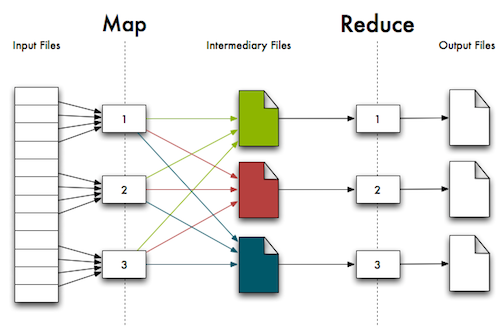
\includegraphics[width=0.8\textwidth]{mapreduce.png}
\caption{Die zwei Phasen eines MapReduce-Jobs \protect\cite{GARFINKEL}}
\label{fig:mapreduce}
\end{figure}

\newpage
\section{Tenzing}

\subsection{Motivation}
Die Autoren des Tenzing-Papers zählen viele Motivations-Faktoren auf. Die wichtigsten werden in den folgenden Abschnitten kurz genannt und erläutert.

\subsubsection{Einfachere Schnittstellen}
Obwohl MapReduce komplexe Berechnungen erfolgreich hinter einem ausgesprochen simplen Programmier-Modell versteckt ist die Einstiegshürde für Nicht-Programmierer doch noch relativ hoch. Im internen Betrieb von Google verlangt die Nutzung des MapReduce-Frameworks ein gewisseses Verständnis von verteilten System sowie C++ und/oder Java.

\subsubsection{SQL-Kompatibilität}
Eng verwandt mit dem Wunsch nach einfacheren Schnittstellen ist die Unterstützung des SQL/92-Standards. Viele Entwickler haben ein profundes Wissen über SQL. Die Akzeptanz von Tenzing ist damit wesentlich größer. Der Einsatz in anderen Gebieten wird dadurch ebenfalls unterstützt.

\subsubsection{Geringe Latenzen}
Klassische MapReduce-Jobs sind in der Lage mit extrem großen Daten umzugehen. In der Regel benötigen diese Berechnungen aber mehrere Minuten, in einzelnen Fällen auch bis zu einigen Stunden. Für effektive statistische Analysen soll Tenzing die Möglichkeit bieten solche Laufzeiten in den einstelligen Sekunden-Bereich zu drücken.

\subsubsection{Effizienz}
Viele heterogene Systeme, die wie Tenzing auf unterschiedlichen Persistenzmechanismen beruhen, entwerfen entsprechende Schnittstellen um Unterschiede wegzuabstrahieren. Tenzing will die diversen Optimierungen der zugrundeliegenden Systeme nutzen. Zu diesem Zweck ist Tenzing so konzipiert, dass Meta-Informationen über die Persistenz-System bekannt sind und vom Query Optimizer berücksichtigt werden können.

\subsubsection{Skalierbarkeit}
Viel Entwicklungszeit ist bei Google bereits in die Entwicklung des Google File Systems sowie des MapReduce-Frameworks geflossen. Beide Technologien sind stark auf massive Skalierbarkeit ausgelegt. Tenzing will sich diese Eigenschaften zunutze machen, indem es auf Basis des MapReduce-Frameworks entwickelt und ausgeführt wird.

\newpage
\subsection{Architektur}
Tenzing besteht aus vier Kern-Komponenten \cite{TENZING}:

\begin{figure}[H]
\centering
\digraph[height=0.7\textwidth]{architecture} {
    node [shape="box"]
    edge [dir="both"]
    client [label="Client Interfaces"]
    query [label="Query Server"]
    meta [label="Metadata Server"]
    pool [label="Worker Pool"]
    data [label="Data"]
    client -> query
    query -> pool
    query -> meta
    query -> data
    pool -> data
}
\caption{Tenzing Achitektur}
\label{fig:architecture}
\end{figure}

\begin{enumerate}
\item \paragraph{Client Interfaces}
Für die Kommunikation mit Tenzing stehen ein Command Line Interface, ein Web User Interface sowie eine API zu Verfügung. Die API bietet die größte Flexibilität während das Web Interface für die meisten Analysten ausreichend ist.
\item \paragraph{Query Server}
Der \textit{Query Server} nimmt Tenzing-Queries an, führt diverse Optimierungen durch und erstellt einen detaillierten Ausführplan.
\item \paragraph{Distributed Worker Pool}
Die Worker im \textit{Distributed Worker Pool} bekommen den Ausführplan eines Queries vom \textit{Query Server} und führen die entsprechenden MapReduce-Jobs aus
\item \paragraph{Metadata Server}
Der \textit{Metadata Server} speichert diverse Metadaten wie zum Beispiel Tabellennamen, Schemas sowie Adressen und Pfade für Dateien.
\end{enumerate}

\newpage
\section{Tenzing im Vergleich}
In diesem Kapitel wird Tenzing mit diversen Systemen und Lösungsansätzen verglichen die eine ähnliche Zielsetzung haben wie Tenzing. Einige dieser Lösungen sind näher am Konzept von Tenzing, andere schlagen einen komplett unterschiedlichen Weg ein. Das Ziel dieser Vergleiche ist es Tenzing hinsichtlich bestimmter Eigenschaften fundierter bewerten zu können.

\subsection{Apache Hadoop}
Das Apache Hadoop Projekt hat es sich zum Ziel gesetzt die Technologien, die in den Papers \textit{MapReduce: Simplified Data Processing on Large Clusters} \cite{MAPREDUCE}, \textit{The Google File System} \cite{GFS} und \textit{BigTable: A Distributed Storage System for Structured Data} \cite{BigTable} beschrieben werden, als Open-Source-Implementierung bereitzustellen. Hadoop ist heute eines der größten Apache Top-Level-Projekte. Für viele Teilbereiche existieren mittlerweile Sub-Projekte die zusammen das Hadoop -Ökosystem bilden. Einige dieser Projekte werden in den folgenden Kapiteln mit Tenzing verglichen.

\begin{figure}[H]
\centering
  \Large
  \renewcommand*\arraystretch{1.1}
  \begin{tabular}{| c | c | c |}
    \hline \textbf{Pig} & \textbf{Hive} & \textbf{Sqoop}\\ 
    Data Flow & Query Language & SQL Import/Export \\ \hline
    \noalign{\smallskip}
    \hline \multicolumn{3}{|c|}{\textbf{MapReduce}} \\ 
    \multicolumn{3}{|c|}{Job Scheduling/Execution System} \\ \hline
    \noalign{\smallskip}
    \cline{1-2} \multicolumn{2}{|c|}{\textbf{HBase}} \\ 
    \multicolumn{2}{|c|}{Column Database} \\ \cline{1-2}
    \noalign{\smallskip}
    \hline \multicolumn{3}{|c|}{\textbf{HDFS}} \\ 
    \multicolumn{3}{|c|}{Distributed File System} \\ \hline
  \end{tabular}
\caption{Das Hadoop-Ökosystem}
\label{fig:hadoop-ecosystem}
\end{figure}

Abbildung \ref{fig:hadoop-ecosystem} zeigt die wichtigsten Teile des Hadoop-Ökosystems. HBase, Pig und Hive werden in den folgenden Kapiteln genauer untersucht. Das \textit{Job Scheduling/Execution System} ist direkt nach dem MapReduce-Paper und das verteilte Dateisystem \textit{HDFS} nach dem \textit{Google File System} \cite{GFS} modelliert. Sqoop hat es sich zum Ziel gesetzt Daten aus relationalen Datenbanken in HDFS zu im- und aus HDFS in relationale Datenbanken zu exportieren. Die typischen Anwendungsfälle von Tenzing und Sqoop unterscheiden sich sehr weshalb Sqoop in diesem Kapitel nicht genauer bearbeitet wird.

\subsection{Apache HBase}
Apache HBase \cite{HBase} gilt als die führende Open-Source-Implementierung der BigTable-Technologie\cite{BigTable}. HBase ist ein \enquote{sparse, distributed, persistent multidimensional sorted Map} \cite{JavaMagazin}. HBase arbeitet also nicht wie traditionelle Datenbanken sondern kann eher als ein mehrdimensionelles, assoziatives Array betrachtet werden. Spalten können beliebig hinzugefügt werden und nicht jede Zeile im Datenbestand muss einen Wert für diese Spalten enthalten. Zusätzlich zu den zwei Dimensionen (Spalten und Zeilen) werden Zellen über Zeitstempel versioniert.

Ähnlich wie das MapReduce-Framework und HDFS arbeitet auch HBase mit einem Master-Server und sogenannten RegionServers. Abbildung \ref{fig:hbase} veranschaulicht die Architektur anhand eines Diagramms. HBase, wie auch BigTable, bietet keine eigene Abfragesprache. Zugriffe auf die Daten laufen über APIs die in vielen verschiedenen Programmiersprachen angeboten werden.

\begin{figure}[H]
\centering
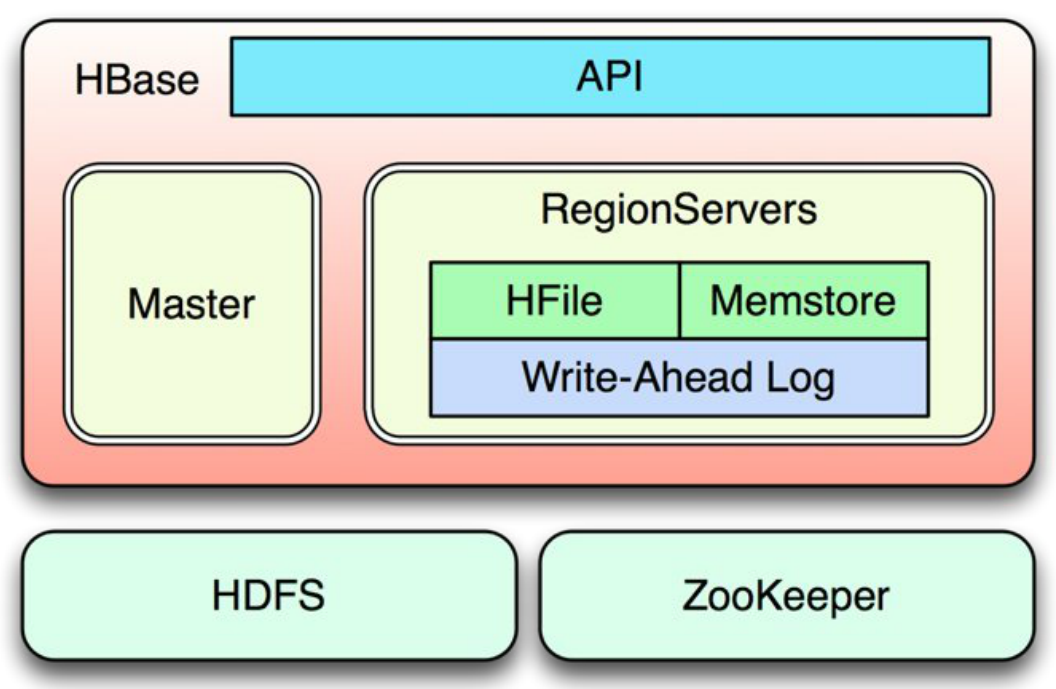
\includegraphics[width=0.75\textwidth]{hbase-architecture.png}
\caption{HBase Architektur \cite{docstoc}}
\label{fig:hbase}
\end{figure}

HBase wäre ein wichtiger Bestandteil einer Open-Source-Variante von Tenzing aber kein eigenständiger Konkurrent oder gleichwertiger Ersatz.

\subsection{Apache Pig}
Im Rahmen des Apache Pig Projektes wurde \textit{PigLatin} entwickelt, eine prozedurale Hochsprache für Abfragen die in MapReduce-Jobs kompiliert wird. PigLatin hat einige Ähnlichkeiten zu Sawzall \cite{Sawzall} das ebenfalls von Google entwickelt wurde. Beide Sprachen sind imperativ wobei ein Sawzall-Programm genau einem MapReduce-Job entspricht währen Pig-Programme in mehrere solcher Jobs kompiliert werden können \cite{PigWiki}. Die Motivation von Pig ist es, MapReduce-Jobs mit weniger Quellcode und dadurch mit weniger Aufwand in kürzerer Zeit zu schreiben \cite{pdfcast}. PigLatin übernimmt eine Sprachkonstrukte und Schlüsselwörter aus dem SQL-Standard was den Einstieg für SQL-Kenner erleichtert.

Pig und Tenzing teilen die Motivation das Analysieren von großen Datenmengen mithilfe von MapReduce zu vereinfachen. SQL und PigLatin sind beides extrem spezialisierte Hochsprachen die es erlauben sehr ausdrucksstark Abfragen zu schreiben. Der Ansatz bei Tenzing, den SQL92-Standard so strikt wie möglich einzuhalten, hat seine Berechtigung wenn man bedenkt wieviele Programmierer und Analysten SQL beherrschen. Nichtsdestotrotz wäre Pig, wie auch HBase, ein wichtiger Bestandteil einer Open-Source-Variante von Tenzing da es MapReduce-Spezifika gegebenenfalls besser unterstützt als SQL.

\subsection{Apache Hive}
Hive beschreibt sich selbst als \textit{data warehouse software [that] facilitates querying and managing large datasets residing in distributed storage} \cite{HiveWiki}. Als Abfragesprache bietet als Hive einen SQL-Dialekt an: Hive-QL oder oft einfach nur QL. Als Data Warehouse System aggregiert Hive Daten aus HDFS-Dateien oder HBase. Eine Eigenschaft die Tenzing und Hive teilen. Ob Hive dabei spezifische Eigenschaften und Optimierungsmöglichkeiten der jeweiligen Datenquellen ausnutzt um die Ausführzeit von Abfragen zu reduzieren war leider nicht zu ermitteln. Generell haben Hive-Queries eine Laufzeit im Minuten-Bereich; Hive ist also nicht für Echtzeit-Abfragen geeignet. Hier spielt Tenzings Worker Pool seine volle Stärke aus da Anfragen Prozesse wiederverwenden und dadurch die benötigte Zeit reduzieren. Zusätzlich bietet Hive, ähnlich wie Tenzing, auch die Möglichkeit über sogenannte \textit{User-Defined Functions} die Sprache um Funktionen und Features zu erweitern. Von den bisher untersuchten System hat Hive, im Vergleich zu Tenzing, die meisten vergleichbaren Ansätze und Eigenschaften. 

\subsection{HadoopDB}
Im Paper \textit{HadoopDB: An Architectural Hybrid of MapReduce and DBMS Technologies for Analytic Workloads} \cite{HadoopDB2009}, veröffentlicht im August 2009 von Forschern der Yale sowie der Brown University, wird ein System vorgestellt das Eigenschaften von parallelen Datenbanken und MapReduce-Frameworks kombiniert. HadoopDB verspricht die Ausfallsicherheit und Skalierbarkeit eines MapReduce-Systems mit der Performance von parallelen Datenbank zu verbinden. Technisch realisiert wurde das System durch diverse Erweiterungen für Hadoop und Hive. Abbildung \ref{fig:hadoopdb} zeigt die Architectur des System. Die blauen Bereiche stellen die HadoopDB-spezifischen Erweiterungen dar. Die Architektur basiert darauf dass jeder Knoten im Cluster eine lokale Datenbank besitzt und MapReduce als Vermittlungsschicht zwischen den Knoten verwendet wird. Offiziell unterstützt HadoopDB MySQL und PostgreSQL. Leider war weder zu ermitteln ob beide Datenbank transparent im gleichen Cluster verwendet werden können noch ob HadoopDB spezifische Eigenschaften dieser Datenbank ausnutzen kann. Die Anbindung von Column Stores, wie beispielsweise HBase, ist in Planung aber noch nicht verfügbar. Auch hier wäre es interessant zu wissen ob HadoopDB ein heterogenes Setup aus Column Stores und relationalen Datenbanken unterstützt. Leider wurden keine schlüssigen Informationen diesbezüglich gefunden.

\begin{figure}[H]
\centering
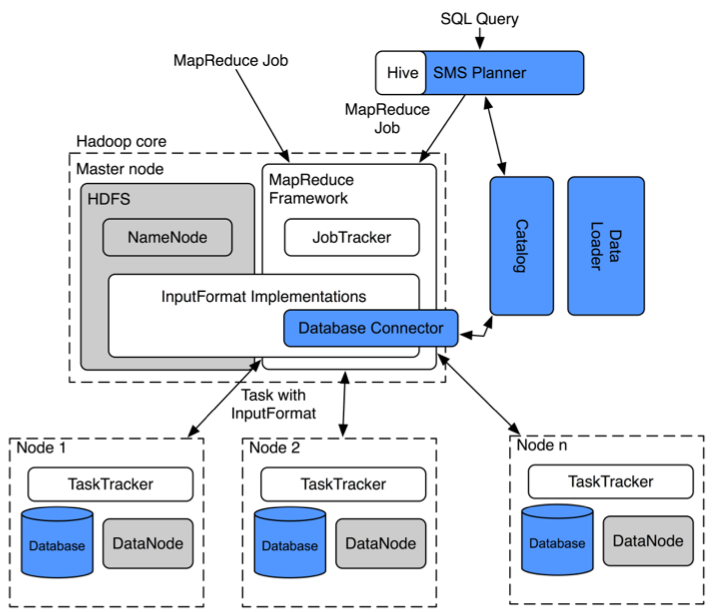
\includegraphics[width=0.8\textwidth]{hadoopdb-architecture.png}
\caption{HadoopDB Architektur \cite{HadoopDB2010}}
\label{fig:hadoopdb}
\end{figure}

HadoopDB scheint viele der Eigenschaften von Hive zu übernehmen, setzt aber gezielt auf eine höhere Performance. Durch das Zusammenspiel von MapReduce und traditionellen Datenbanken entsteht ein hybrides System das an vielen Stellen an Tenzing erinnert. Falls die Unterstützung unterschiedlicher DBMS und gegebenenfalls sogar die Integration von Column Stores innerhalb eines Clusters geplant ist hätte HadoopDB bezüglich heterogener Datenquellen große Ähnlichkeiten mit Tenzing.

\newpage
\subsection{Nephele und PACT}
Die Technische Universität Berlin hat 2011 einen wissenschaftlichen Forschungs-Artikel mit dem Titel \textit{MapReduce and PACT - Comparing Data Parallel Programming Models} \cite{PACT} veröffentlich. Darin wird die Nephele Execution Engine sowie das PACT Programmiermodell vorgestellt. Nephele basiert auf Hadoop und PACT sieht sich selbst als Erweiterung des MapReduce-Paradigmas. Tenzing und PACT haben einige Gemeinsamkeiten was die Motivation betrifft, verfolgen jedoch grundverschiedene Ansätze bei der Umsetzung. Die Autoren des PACT-Papers stimmen mit der Meinung der Autoren des Tenzing-Papers überein, dass das Schreiben von MapReduce-Jobs aufwändig ist und viele Anwendungsfälle nicht ohne weiteres in MapReduce ausgedrückt werden können. Während Tenzing mit kompletter Unterstützung des SQL-Standards versucht den Zugang zur Analyse von großen Datenmengen zu ermöglichen verfolgt PACT klar den programmatischen Ansatz. 

\begin{figure}[H]
	\centering
	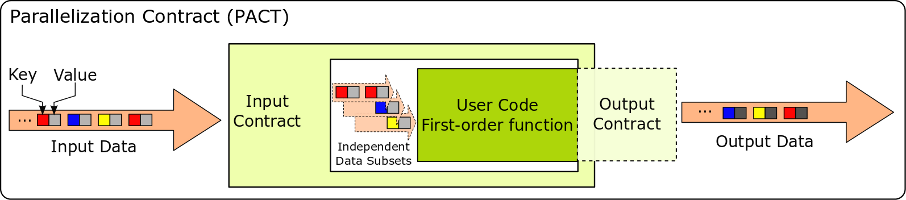
\includegraphics[width=\textwidth]{pact.png}
	\caption{Ausführung eines PACT-Programms}
	\label{fig:pact}
\end{figure}

PACT erweitert das MapReduce-Konzept an zwei Stellen. Neben \texttt{Map} und \texttt{Reduce} wurden drei weitere grundlegende Funktionen identifiziert die für die Analyse von Daten wichtig sind: \texttt{Match}, \texttt{Cross} und \texttt{CoGroup}. 

\begin{enumerate}
    \item \paragraph{Match}
	Die Match-Funktion arbeitet auf Paaren von Schlüssel-Werte-Paaren und kombiniert Paare mit dem gleichen Schlüssel.
	\begin{figure}[H]
		\centering
		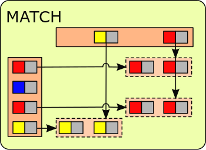
\includegraphics[width=0.5\textwidth]{match.png}
		\caption{Match-Funktion}
	\end{figure}
    \item \paragraph{Cross}
	Die Cross-Funktion bildet Paare von Schlüssel-Werte-Paaren in Form eines kartesischen Produkts. Eigenschaften der Schlüssel, wie beispielsweise die Gleichheit werden nicht beachtet.
	\begin{figure}[H]
		\centering
		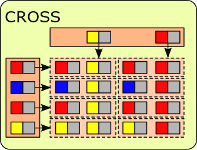
\includegraphics[width=0.5\textwidth]{cross.png}
		\caption{Cross-Funktion}
	\end{figure}
    \item \paragraph{CoGroup}
	Die CoGroup-Funktion arbeitet ähnlich wie Match-Funktion, allerdings bildet sie nicht nur Paare, sondern Gruppen von Schlüssel-Werte-Paaren mit dem gleichen Schlüssel.
	\begin{figure}[H]
		\centering
		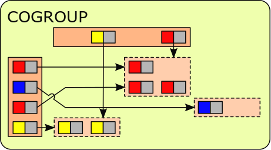
\includegraphics[width=0.5\textwidth]{cogroup.png}
		\caption{CoGroup-Funktion}
	\end{figure}
\end{enumerate}

Im Gegensatz zu Map und Reduce arbeiten die drei zusätzlichen Funktionen immer mit zwei Eingabemengen. Dadurch lassen sich Joins wesentlich einfacher formulieren als mit klassischen MapReduce-Programmen. Zusammen mit Map und Reduce lassen sich diese fünf Funktionen in beliebiger Konstellation zusammenstellen. Während man bei MapReduce auf die starre Abfolge von Map und Reduce angewiesen war, erlaubt es PACT komplexe Analsysen in kleinere und dadurch wiederverwendbarere Bausteine aufzuteilen. Dadurch entsteht in gerichteter Graph der dann von der Execution Engine analysiert und gegebenenfalls optimiert wird. Abbildung \ref{fig:pact} zeigt das Übersetzen eines PACT-Programms in einen ausführbaren Plan.

Nephele/PACT und Tenzing verfolgen extrem unterschiedliche Ansätze für die Lösung des gleichen Problems. Nephele/PACT ist kein Open-Source-Ersatz für Tenzing aber eine vielversprechende Basis für einen Open-Source-SQL-Engine auf Basis von Hadoop. Durch den bereits vorhandenen Compiler und Optimizer fehlt dem Nephele/PACT-System effektiv nur noch eine entsprechende SQL-Schnittstelle. Also eine Komponente die SQL-Queries parsen und in PACT-Programme übersetzen kann. Den aufwändigen Teil des Optimierens und Verteilens bietet das System bereits. 

\begin{figure}[H]
\centering
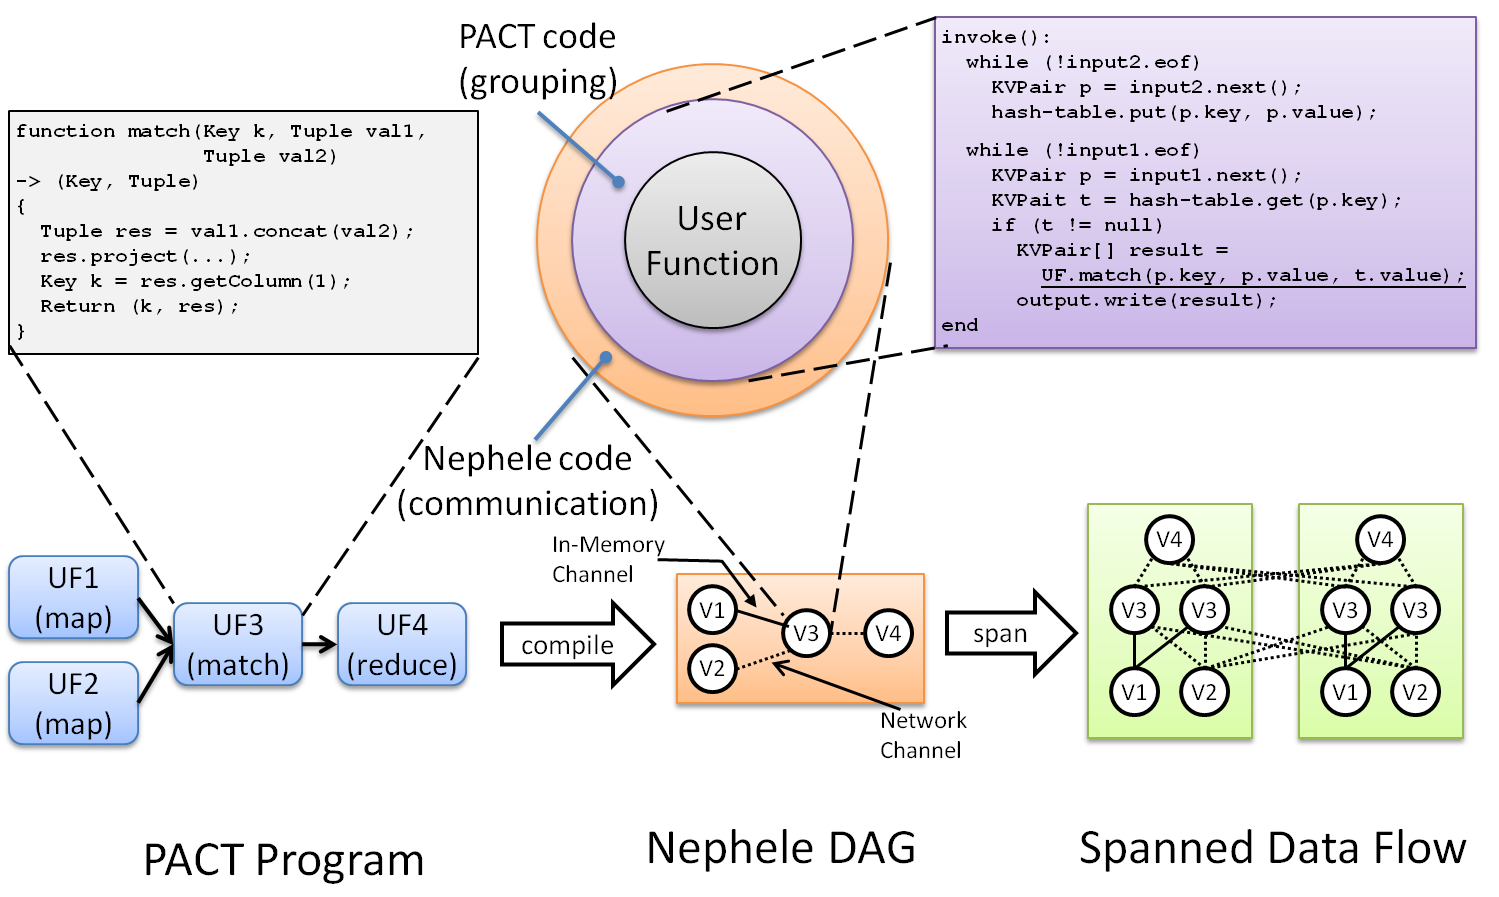
\includegraphics[width=\textwidth]{compilation.png}
\caption{Lebenszyklus eines PACT-Programms}
\label{fig:pact}
\end{figure}

\subsection{Fazit}
Aufgrund der Tatsache, dass der Artikel über Tenzing erst im September 2011 erschienen ist, ist es nicht weiter überraschend, dass es zum aktuellen Zeitpunkt keine Open-Source-Varianten von Tenzing gibt. Nichtsdestotrotz bieten sowohl Hive als auch HadoopDB bereits ausgesprochen ausgereifte Varianten von SQL-Engines auf Basis des Hadoop-Ökosystems an. Zusätzlich wurde im vorherigen Kapitel eine erfolgsversprechende, alternative Route aufgezeigt wie eine Open-Source-SQL-Engine auf Basis von Hadoop entwickelt werden könnte.

\newpage
\section{Eigener Ansatz}
In diesem Kapitel wird ein eigener Ansatz sowie die Idee und Architektur für einen Prototypen vorgestellt. Der Prototyp besteht aus einem eigenen SQL-Dialekt sowie einer Engine die Abfragen in diesem Dialekt in einen MapReduce-Job für das Hadoop-Framework übersetzt.

\subsection{SQL-}
Der SQL-Dialekt \textit{SQL-} (in Worten \textit{SQL Minus}), ist eine extrem kleine Teilmenge von SQL. Es werden ausschließlich Projektion und eine einfache Gruppierung mit einer Aggregation pro Abfrage. Als Aggregatfunktionen werden \texttt{SUM} und \texttt{AVG} unterstützt. Die folgenden Listings zeigen kompatible Queries. 

\begin{listing}[H]
\begin{minted}{sql}
SELECT year, population
FROM hdfs://countries.csv
\end{minted}
\caption{SQL- Select-Syntax}
\end{listing}

\begin{listing}[H]
\begin{minted}{sql}
SELECT country, AVG(population)
FROM hdfs://countries.csv
GROUP BY country
\end{minted}
\caption{SQL- Group-by-Syntax}
\end{listing}

\begin{listing}[H]
\begin{minted}{sql}
SELECT year, SUM(population)
FROM hdfs://countries.csv
GROUP BY year
\end{minted}
\caption{SQL- Group-by-Syntax}
\end{listing}

\begin{listing}[H]
\begin{minted}{sql}
SELECT year
FROM hdfs://countries.csv
GROUP BY year
\end{minted}
\caption{SQL- Group-by-Syntax}
\end{listing}

Abbildung \ref{fig:sampledata} zeigt die Beispieldaten auf die sich die oben vorgestellten Abfragen beziehen können. Konkrete Daten sind beispielsweise auf Geohive.com \cite{GeoHive} verfügbar, was für den Test des Prototypens interessant wird.

\begin{figure}[H]
\centering
\begin{tabular}{l l l}
	\toprule
	country & year & population \\
	\midrule
	DE & 1900 & 56,400,000 \\
	UK & 1900 & 41,600,000 \\
	IT & 1900 & 32,400,000 \\
	... \\
	DE & 1950 & 50,800,000 \\
	UK & 1950 & 50,200,000 \\
	IT & 1950 & 46,800,000\\	
	... \\
	\bottomrule
\end{tabular}
\caption{Beispieldaten}
\label{fig:sampledata}
\end{figure}

\subsection{Schema}
Es gibt zwei Gründe warum die Definition eines Schema der Eingabedatei sinnvoll ist. Einerseits müssen die Spaltennamen, die im Query verwendet werden, auf konkrete Spalten in der Eingabe abgebildet werden, andererseits sind die beiden Aggregatfunktionen nur für numerische Werte definiert. Das erste Problem würde sich durch eine kleine CSV-Datei lösen lassen die nur die Namen der Spalten enthalten. Spaltennamen werden in derselben Reihenfolge angegeben wie die Spalten in der konkreten Eingabedatei. Da die Aggregatfunktionen die einzige Stelle sind an der Datentypen eine Rolle spielen reicht es aus wenn die Umwandlung von Strings in Longs an dieser Stelle passiert.


\subsection{Command Line Interface}
Bedient werden soll der Prototyp über die Kommandozeile in Form eines Command Line Interface. Benutzer der MySQL-Shell werden sofort gewollte Ähnlichkeiten feststellen.

\begin{listing}[H]
\begin{minted}{sh}
java -jar de.bht.pat.tenzing.Main
> SELECT year FROM hdfs://countries.csv
+---------------+
| year          |
+---------------+
| 1950          |
| 1950          |
| 1950          |
| 1951          |
| 1951          |
| 1951          |
+---------------+
6 rows in set (1 min 12 sec)
>
\end{minted}
\caption{Command Line Interface}
\label{lst:cli}
\end{listing}

\subsection{Architekturelle Herausforderungen}
Zwei Teilaspekte des Prototypen erfordern ein genaues Planen, Einschätzen des Aufwandes sowie Abwägen von Alternativen. Der erste Aspekt betrifft das Parsen des SQL-Dialekts in eine verwertbare Struktur. Formal korrekt wäre die Definition einer Grammatik, vorzugsweise in Backus-Naur-Form, und das Erstellen eines Parsers mithilfe eines Parser Generators wie zum Beispiel ANTLR. Aufgrund mangelnden Vorwissens wird von dieser Strategie Abstand genommen. Eine Alternative für das Parsen wären Regulären Ausdrücke. Obwohl Reguläre Ausdrücke ein sehr mächtiges Werkzeug sind erscheinen sie für die Aufgabe doch zu fehleranfällig und nicht ausdrucksstark genug. Um den zeitlichen Aufwand in Grenzen zu halten wird versucht einen bestehenden Open-Source SQL-Parser \cite{SQLParser} für Java zu verwenden.

Der zweite Aspekt der das Potential hat kompliziert zu werden ist die Tatsache, dass die Hadoop-API die Map- und Reduce-Funktionen in Form von Klassen und nicht als Instanzen akzeptiert. Konkret heißt das, dass die übergebenen Mapper und Reducer bereits zur Compiletime existieren müssen, da sie serialisiert und über das Netzwerk im Cluster verteilt werden müssen. Wie die Verwendung eines Parser Generators für den SQL-Dialekt gibt es auch hier eine Lösung die vermutlich die \textit{formal} korrekt wäre aber zu aufwändig ist: die Verwendung eines Bytecode-Generators \cite{Bytecode}. Stattdessen lässt sich die Simplizität des SQL-Dialekts ausnutzen. Es gibt nur zwei Varianten einer Projektion, mit und ohne Gruppierung. Falls in der Selektklausel keine Aggregatfunktion vorkommt reichen ein Mapper und ein Reducer: \texttt{SelectMapper} und \texttt{NoopReducer}. Der SelectMapper liefert nur die gewünschten Spalten, der NoopReducer gruppiert nach Schlüssel, wendet aber keine Aggregatfunktion an. Für den Fall dass in der Projektion eine Aggregatfunktion auftaucht wird wird ein spezieller Mapper, der \texttt{GroupByMapper}, und zwei spezielle Reducer, \texttt{SumReducer} und \texttt{AvgReducer}, benötigt. Da die entsprechenden Klassen bereits zur Compiletime existieren müssen ist es nötig Laufzeitinformationen wie die konkrete Liste der Spaltennamen etc. dynamisch im Cluster zu verteilen. Dazu lässt sich die Hadoop-Klasse \texttt{Configuration} verwendet die es erlaubt beliebige Konfigurationsparameter beim Start festzulegen, die dann für alle Knoten im Cluster verfügbar sind.

\newpage
\nocite{GOOGLE-TENZING}
\nocite{GOOGLE-MAPREDUCE}
\nocite{GOOGLE-GFS}
\nocite{KemperEickler}
\nocite{KandziaKlein}
\nocite{Selinger}
\nocite{Zeller}
\nocite{Ioannidis}
\addcontentsline{toc}{section}{Literatur}
\printbibliography

\newpage
\addcontentsline{toc}{section}{Abbildungsverzeichnis}
\listoffigures

\addcontentsline{toc}{section}{Tabellenverzeichnis}
\listoftables

\addcontentsline{toc}{section}{Quellcodeverzeichnis}
\renewcommand\listoflistingscaption{Quellcodeverzeichnis}
\listoflistings

\end{document}

